To have a better understanding of the desired functionality of our language, we define several use cases that our
solution may be applied to.

Throughout this section we will be defining specific functions that we envision being used, and what must be exposed to
comfortably support them.
It should be noted that for many use cases, we will be drawing from real world algorithms, as for most of these
algorithms there already exist solutions - our goal will not be to implement them ourselves, but to provide a platform
where they can be executed.
For example, in~\ref{subsec:naive-pathfinding} we cover our need for a pathfinding algorithm, here we are referring to
being able to build a domain where the information can exist, in reality our implementation would simply use an
existing search algorithm given the structure that the user has created.

\subsection{Minimum Viable Product}\label{subsec:minimum-viable-product}
For the language to be usable it must implement basic types and operations, as the focus of the language, graphs must
exist as a data type that can be created and modified.
Ideally our MVP would include a turing complete~\cite{TuringCompleteness} suite of operations, allowing users to take
advantage of supported functionalities, while still having the ability to build ad-hoc unsupported features.

\begin{figure}[H]
    \centering
    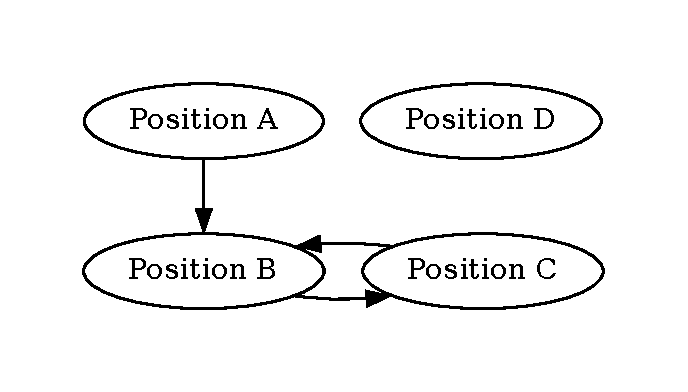
\includegraphics[width=12cm]{figures/example_graphs/basics.gv}
    \caption{An example of a graph displaying each of the most basic features that we expect to implement}
    \label{fig:example_basic_graph}
\end{figure}

Figure~\ref{fig:example_basic_graph} covers the three types of relationships we are expecting to come across.
Our first graph based feature would naturally be to find some way to visualize the graph that we have built, similar to
the generated figure.

\subsection{Naive Pathfinding}\label{subsec:naive-pathfinding}
One of the more fundamental sets algorithms in computing, we expect a finished product to support some level of node
navigation and optimisation.

\begin{figure}[H]
    \centering
    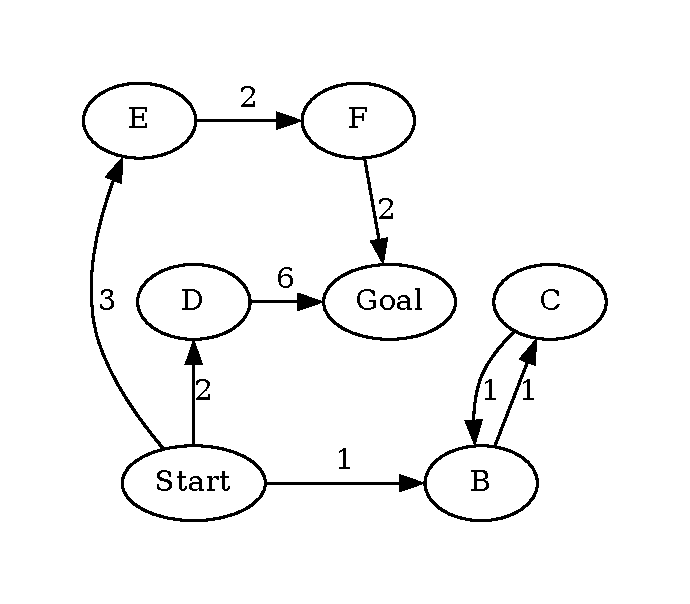
\includegraphics[width=12cm]{figures/example_graphs/pathfinding.gv}
    \caption{An example of a graph that needs to be navigated through}
    \label{fig:example_pathfinding_graph}
\end{figure}

Figure~\ref{fig:example_pathfinding_graph} defines a graph that has a starting node and a goal node, with edges
simulating the cost of traversing between nodes.
Our intent when implementing pathfinding support is to provide a framework where a user can build such a graph, and
given an arbitrary start node, goal node, and algorithm, will be able to retrieve the cost and path that is outputted by
the algorithm.
One important note when implementing such a functionality is that pathfinding algorithms assume a cost of node
traversal, if we build a generalised solution we will have to ask ourselves how this cost should be implemented, as we
have multiple options:

\textbf{All edges have costs, defaulting to 0}~-~this approach allows us to run pathfinding algorithms on any graph, and
requires very little work from a programmer to ensure the graph remains compliant.
However, there are arguments to be made for wasted allocated memory on larger graphs that have no need for such a value.

\textbf{Different subclasses of graphs}~-~this approach would allow us to define a type of graph that MUST have a cost,
while it prevents useless memory allocation, it also requires more work on the side of the developer, who must both
learn and remember the arbitrary definition we have created.

\textbf{Algorithms that treat undefined costs as 0}~-~while this approach may seem more elegant, as it avoids both
previously listed issues, it also introduces implicit functionality, which may produce confusing results if developers
expect a different behaviour when attempting to use pathfinding on non-compliant graphs.

\subsection{Constraint Satisfaction}\label{subsec:constraint-satisfaction}
Constraint satisfaction Problems (CSPs) allow developers to create nodes as a set of domains that can then be reduced.
Creating a graph that needs to be constrained requires us to define two features - a node must be comprised of a domain
of possible values (that will then be constrained); and the constraint itself must exist as part of the relationship.
Unary constraints must also be taken into consideration, as they do not require a relationship to exist.

\begin{figure}[H]
    \centering
    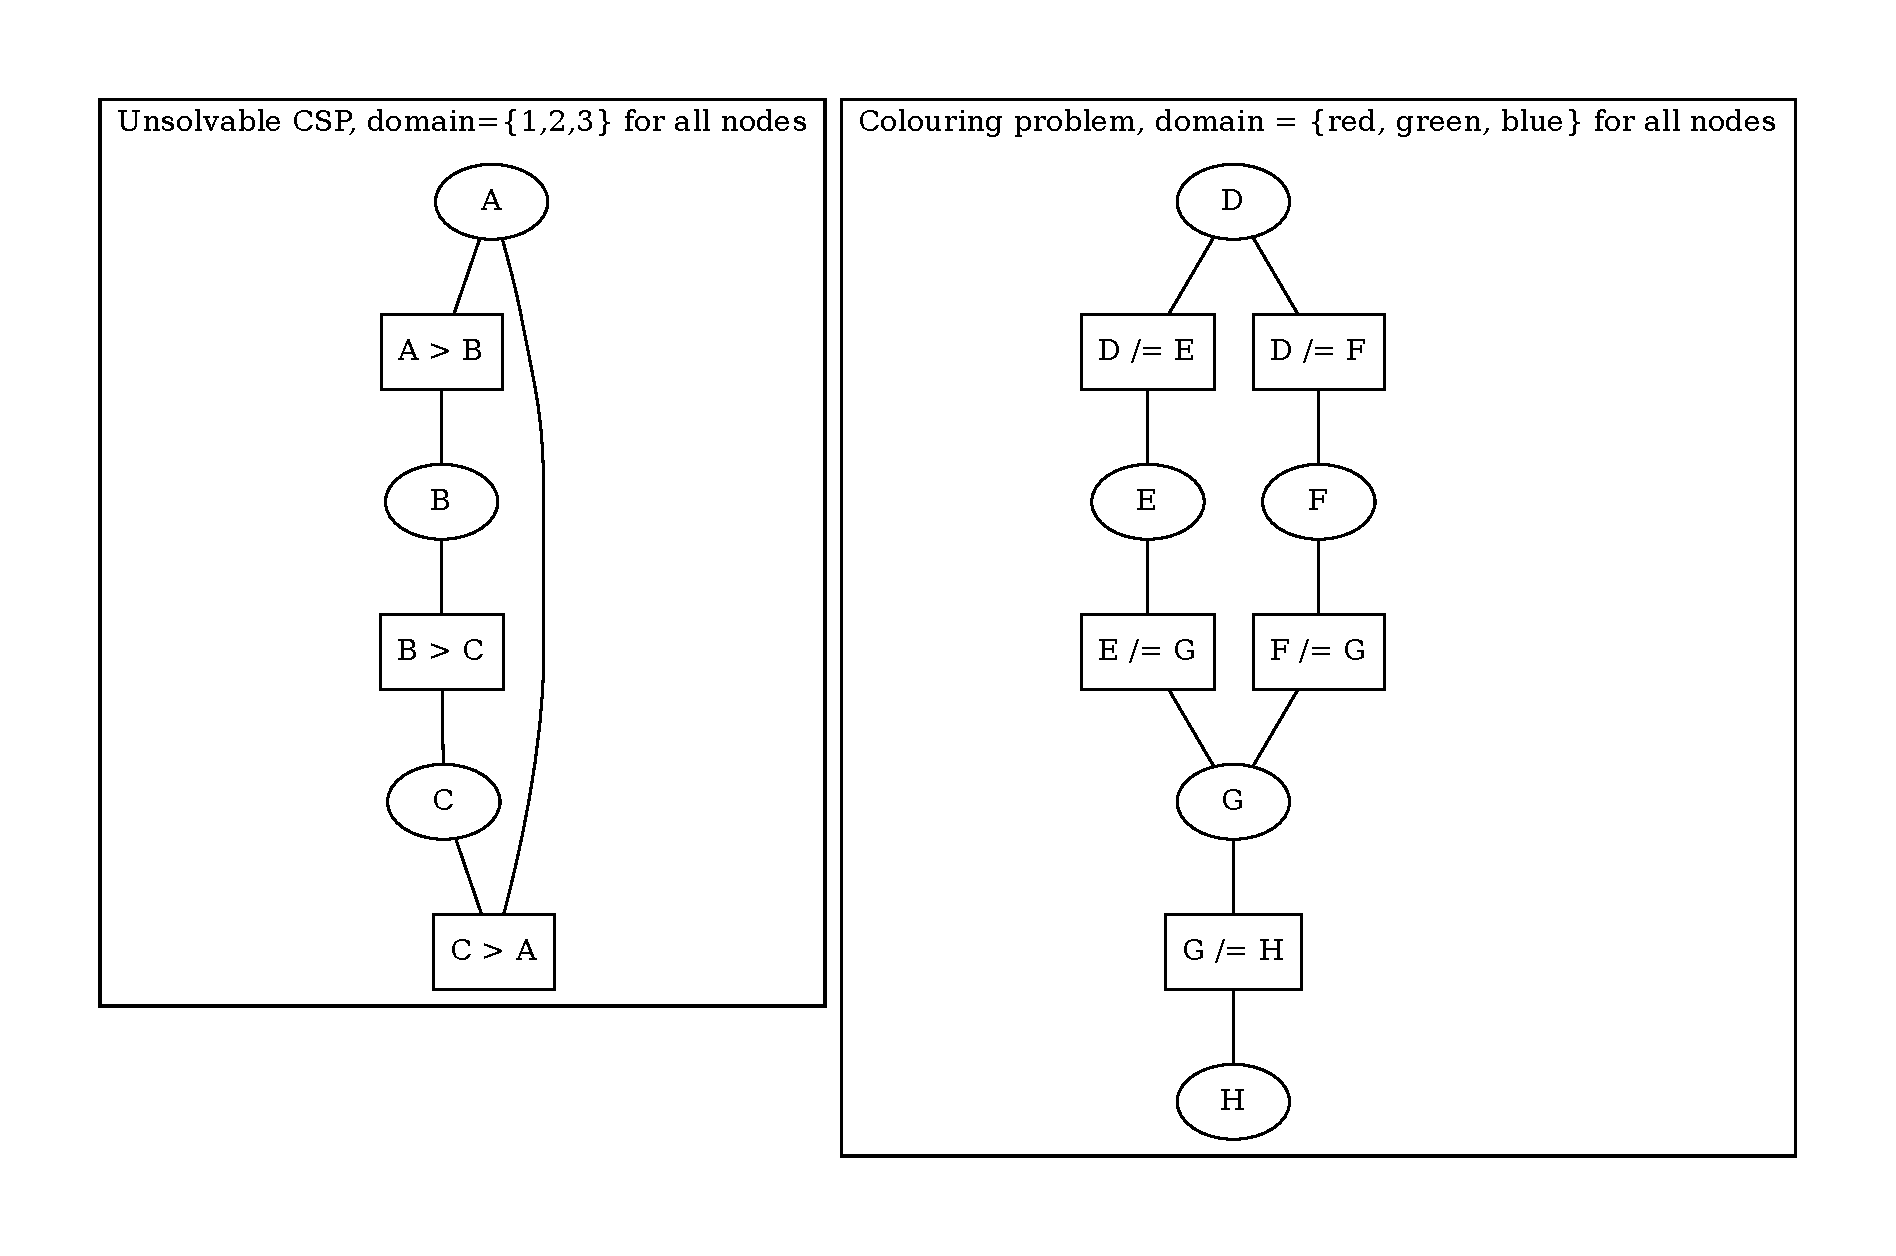
\includegraphics[width=12cm]{figures/example_graphs/constraint_satisfaction.gv}
    \caption{An example of a graph has constraints that need to be acted upon}
    \label{fig:example_constraint_graph}
\end{figure}

In Figure~\ref{fig:example_constraint_graph} we define two separate graphs that can be constrained.
Our first consideration for the first graph is how our language should respond to situations where constraints can not
be met, we will discuss this in further detail during the implementation section.
Next, we approach a more realistic constraint problem with applicable algorithms to find a list of ``correct'' answers.
Here we run into similar questions as were raised in pathfinding, how do we handle knowing whether a graph is compliant
with required format for CSP algorithms?

Lastly we introduce the possibility of interoperability between constraint satisfaction and other language features.
As constraints remove items from a domain, we can introduce the concept of changing or adding constraints as a form
of modifying existing data.
A common use case may be that to remove a node, it would simply have a unary constraint applied to it which is always
False - alternatively it may make more sense to introduce variable elimination functionality to ensure that changes
remain predictable.

\subsection{Trees}\label{subsec:trees}
Trees can be considered a subset of graphs, in that they limit the way relationships can be formed.
Earlier we mentioned the possibility of inherited types that can be used to ensure specific structures - for trees we
believe that this distinction is necessary, as it is a significant departure from what a graph can represent.

\begin{figure}[H]
    \centering
    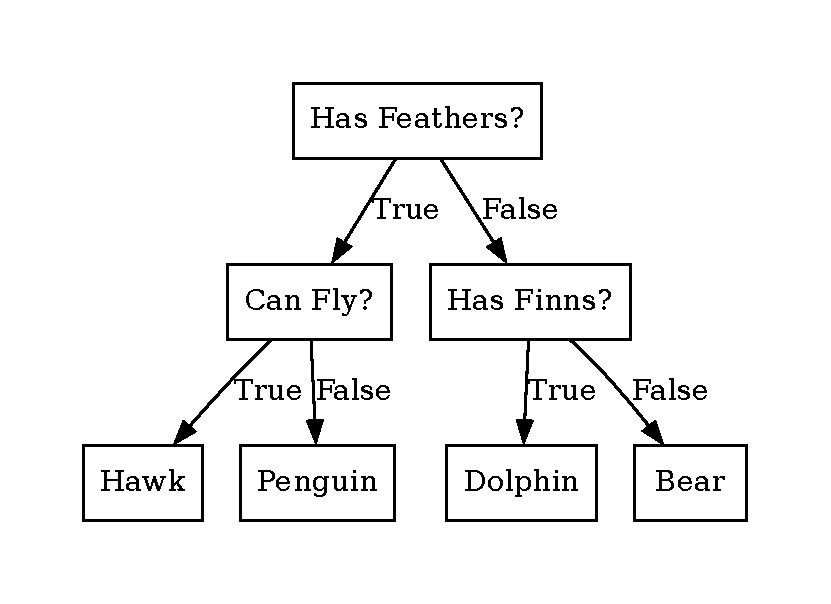
\includegraphics[width=12cm]{figures/example_graphs/decision_tree.gv}
    \caption{An example of a decision tree that could be represented in our language}
    \label{fig:example_decision_tree}
\end{figure}

In figure~\ref{fig:example_decision_tree} we define a basic tree structure, logically, it appears that the only
consideration we will have when building this structure is to ensure that nodes may only be added or removed in a
certain way.
Unlike previous sections we do not run into ill-formed algorithms here, any solution that applies to the previous
sections will be inherited into this section.

\subsection{Supplementary Use Cases}\label{subsec:supplementary-use-cases}
Having covered some more simple and common use cases of graphs we can start looking into more obscure and complex
cases.
We will use the following examples not just to fill in features with excess time, but to have a better idea of the
more complex applications that we intend from our language - thus we look for use cases that may help inspire
generalised base functionality.

\subsubsection{Informed Search}
Informed search introduces the concept of heuristics to optimise the number of nodes a search algorithm must explore.
Heuristics act as pieces of metadata that can be used to infer which node of the algorithm's frontier is most likely 
moving more efficiently towards the goal - in order to implement them we can consider two approaches:

\textbf{Metadata tags}: This approach would require search algorithms to access such a tag on each node of a frontier,
this may be inefficient if the goal node of the graph is expected to change (different goal nodes will generate
different sets of heuristics)
\textbf{Heuristic graphs}: With this approach an overlying graph of the heuristic costs would have to be generated,
while there are questions to be raised about efficiency of creating potentially an exponential number of graphs, our
primary concern is with the process of overlaying one graph across another.
This includes an additional property that we may build traversal optimisations which result in the heuristics graph
becoming a subset of the graph that the algorithm is being applied to.

\subsubsection{Bayesian Networks}
Bayesian networks are a probabilistic model that allow users to make analysis of how events affect each other.
Similar to CSPs, this use case would have nodes representing a specific domain of values (truth tables in this case) -
the reason we introduce this as a possibility is to raise the question of how algorithms expecting specific types of
domains should be treated.
In the case of CSPs, we can simply attempt to run the constraint on any iterable values, however bayesian networks
introduce the idea that we may have domains that are slightly harder to validate, possibly requiring us to have
specific node types set aside for such use cases.

\subsubsection{Neural Networks}
We explore neural networks mainly for the concept of ``hidden layers''~\cite{NNetHiddenLayers} - to simulate a neural
network, we must be able to programmatically build nodes that are not directly accessible to the developer.
This raises questions for traversal, for example if there is a relationship of nodes
\textbf{N1 -e1> h1 -e2> h2 -e3> N2}, where h1 and h2 are ``hidden'' nodes, how would the edge e2 ever be updated?
To tackle traversal and access issues, we will have to take a deeper look into how we expect developers to access nodes
and relationships of a graph, and how we believe they would run operations given that information.

\subsubsection{Network Topology}
Network topology differentiates from regular graphs in that we expect nodes to be individual units that each can do
work.
The concept that we introduce with network topology is that the nodes are individual functioning units that carry out
their own operations - susceptible to failure irregularity.
Considerations of this use case may lead us to conclude that nodes and relationships require even heavier abstraction,
where nodes can carry out multithreaded functions within the graph, and relationships represent a more accessible
entity, such that a simulation of a real world network could be simulated in our language.

\subsubsection{Graph Databases}
Finally, we choose graph databases as an interesting use case as a real life implementation of a graph database would be
unable to store all existing data in memory.
We should keep this use case in mind when considering how graphs should be saved/loaded, and explore solutions to
prevent overuse of memory when nodes are accessed.
Furthermore, we should include existing graph databases as research into the application of our language, as the formats
for querying and storing data may be congruous with other use cases we have defined.

\subsection{Feature Wishlist}\label{subsec:feature-wishlist}
In conclusion to covering use cases we can draw a prioritised list of features that we would want to include in our
language, this will help us with our preliminary research into the tools and approaches we will need to implement.

The features as a rough overview are as follows:
\begin{itemize}
    \item Basic language functionalities
    \item The ability to build a graph data type with Nodes connected by Edges
    \item Functionality to apply basic CRUD operations on nodes and edges
    \item Functionality to find optimal paths between nodes
    \item Functionality to constrain nodes by building constraints along edges (or on nodes for unary constraints)
    \item Inherited reduced functionality graphs designed for specific algorithms/use cases
\end{itemize}

We can also list the supplementary features we have outlined:
\begin{itemize}
    \item Graphs that may overlay over each other for multidimensional algorithms
    \item Fixed domain graphs when specific types of domains are expected
    \item Hidden nodes that are programmatically built with the intention of not being accessed directly
    \item Nodes that define their own functionality, perhaps even running their own multithreaded operations
    \item The ability to access parts of the graph in-memory, preventing all data from being loaded at once
\end{itemize}